\subsection*{Overview}
After the sliding window code was run on Figure \ref{fig:fruit} in experiment 8,
it was observed that a sliding window was predicting grapes correctly in
regions that contained a bunch of grapes. Since it would make sense that the
model would be able detect an individual grape, it was decided that I would run
recursive refinement on a window that contained a grape. Due to the model
requiring a 299 x 299 image size, the window could only be refined once as
very small segments could not be resized up to 299 x 299. I decided to use a
window of 70 x 70.

\subsection*{Script}
As you would think with recursive refinement, a recursive function would used,
but I found this unnecessary due to image size restrictions. Instead, a
conditional for loop was added to the existing code.
\begin{lstlisting}
if top1 == "grape" and window_shape == "grid" and rr_grape:
			for (x_grape, y_grape, grape_window) in sliding_window(window_resized, stepSize=64, windowSize=(70, 70)):
				#reshape to square
				grape_window_resized = cv2.resize(grape_window, (299, 299))
				top1_grape = subSample.classify(grape_window_resized, window_shape)
				if top1_grape == "grape":
					cv2.rectangle(display_image, (x_grape + x, y_grape + y), (x_grape + x + 70, y_grape + y + 70), colour_dict.get(top1, (0,0,0)), 4)
					#cv2.imshow("Window", grape_window_resized)
					cv2.waitKey(1)
time.sleep(0.025)
\end{lstlisting}

\begin{figure}
    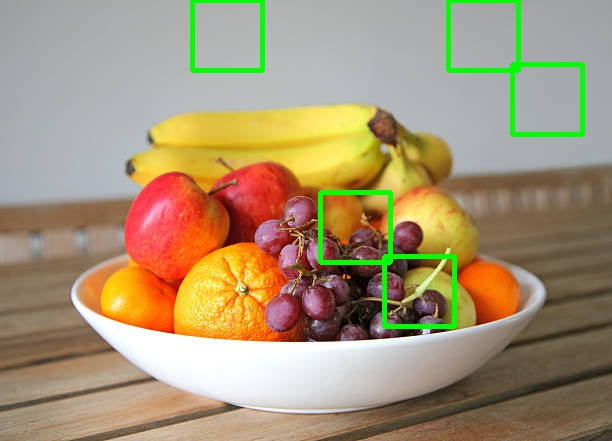
\includegraphics[scale=0.5]{fruit_rr}
      \caption{Recursive refinement 1}
      \label{fig:rr1}
\end{figure}

\begin{figure}
    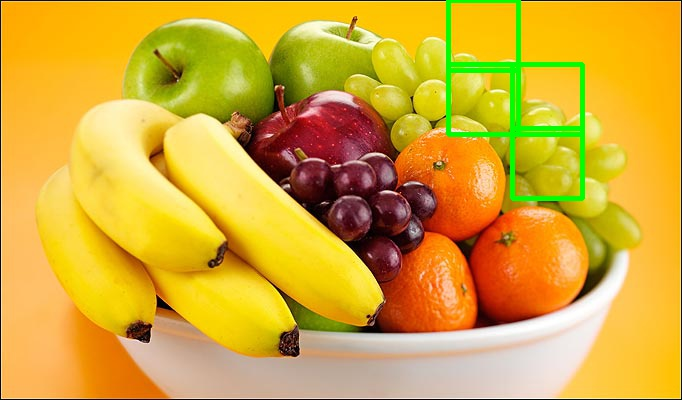
\includegraphics[scale=0.5]{newfruit_rr_grid}
      \caption{Recursive refinement 2}
      \label{fig:rr2}
\end{figure}

\begin{figure}
    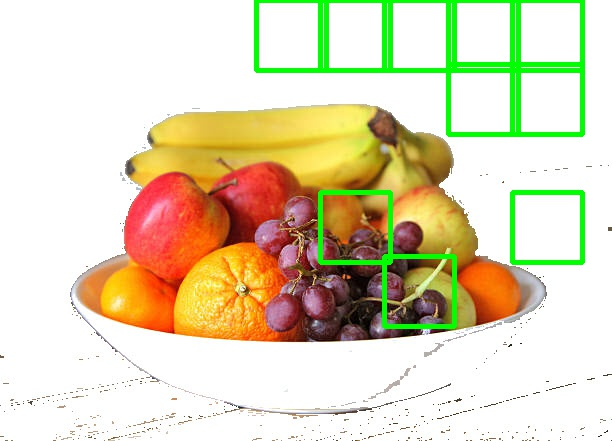
\includegraphics[scale=0.5]{processed_image}
      \caption{Recursive refinement 3}
      \label{fig:rr3}
\end{figure}


\subsection*{Results}
Some very interesting results on three separate images. Two new images are seen
here which we will explore in future experiments. In all three images, while we
are getting some expected predictions, grapes are being classified in locations
that have nothing resembling a grape. These can be viewed in Figures
\ref{fig:rr1}, \ref{fig:rr2} and \ref{fig:rr3}.

\subsection*{Analysis}
